\chapter{Collection Server}
\label{chap:mmeasurement}
To collect only dates relevant for the purpose of the survey and its safe transmission, the client has a major role. The server however, is also important for keeping the data safe and consistent. Without correctly handled data processing, the best collection software is meaningless.\\
The timely decryption and decoding of the incoming data are of the same importance as the correct storage solution for the amount of expected information.

While we discussed the client-side in the last chapter, this chapter is going to focus on
the server-side implementation of the data collection process. 
We are giving some general recommendations again in the first section and talk more in-depth about our implementation in section \ref{sec:measurement:eval_setup}.
%


%%%%%%%%%%%%%%%%%%%%%%%%%%%%%%%%%%%%%
%%%%%%%%%%%%%%%%%%%%%%%%%%%%%%%%%%%%%
%%%%%%%%%%%%   SECTION   %%%%%%%%%%%%
%%%%%%%%%%%%%%%%%%%%%%%%%%%%%%%%%%%%%
%%%%%%%%%%%%%%%%%%%%%%%%%%%%%%%%%%%%%
\section{General recommendations}
    \label{sec:measurement:limits}
%
    As every setup and organization is different, we provide some general recommendations and the reasoning behind each step. We discuss steps to reduce the attack surface of the server, as well as storage best practices. Furthermore we showcase database performance and how to prevent command injections.
    
    \subsection{Data security}
        \label{subsec:data_storage}    
        If no additional PII was collected, the only information, which could be used for re-identification is the ID, which should be anonymized sufficiently during the collection process. If you plan on releasing at least parts of the gathered data with the ID included, an additional step could be the encryption with a key and salt that is only known to the server before storing the ID locally. That way, the privacy of the user is further enhanced. Someone who gains access to the data can no longer connect any data in transit with the stored data that way.
        To avoid that an attacker may obtain the key or salt, proper access restrictions should be in place, and the server kept up to date.\\
        To reduce the speed and success rate of user enumeration and login brute-forcing attempts intrusion protection systems like \textit{fail2ban} \cite{noauthor_fail2ban_nodate} can be deployed. These tools apply defined rules to firewalls or webservices base on log file events. All services that don't need to be internet facing should be isolated by firewall rules or kept on separate networks. This reduces the attack surface of the server. The probability of vulnerability that allows unauthorized access is increased with each internet facing service.\\
        As of Smithsonian recommendation, it should be documented who may have access to the data \cite{noauthor_best_2018}. Following their recommendations, it should also be documented who is responsible for the data in which phase of the life-cycle. This is important to trace data in case of leakage or a member leaves the project and some one has to take over the responsibilities.\\
        Data backups should follow the 3-2-1 rule. Keep at least 3 stored copies on two different media with at least one off-site location. This helps to prevent data loss in case of a failure or attack.
        Furthermore, a project should specify the lifetime of data before it gets deleted. If it is planned to archive the data for an extended period, it should be documented where the archive is stored \cite{noauthor_best_2018}. That way, it is clearly stated for the processing people, where backups are stored which might need be destroyed as well.
        Further information on how to secure access can be reviewed in NIST's Security Guidelines for Storage Infrastructure \cite{chandramouli_security_2020}. \\
        Another possibility is to store the data encrypted to decouple the private key from the collection server, which increases the overhead for evaluation of the data. On the other hand, an adversary has fewer gains from a successful attack. Especially if the ID is encrypted as well before storing it.\\
        While this procedure might increase the users' trust in the collection process if known publicly, the gains and overhead should be weighed against each other. If no additional PII is collected, the encryption of statistical data might just add overhead without adding any significant gain.
        
\newpage
    \subsection{Databases} 
        \label{subsec:database}
        For relational databases, we would recommend PostgreSQL \cite{group_postgresql_2021}.
        It proved to be faster than MongoDB \cite{makris_mongodb_2020} in almost all cases and performed better against OrientDB and Neo4j in almost all operations \cite{noauthor_benchmark_2018}. It was second to none in  \cite{noauthor_benchmark_2018} when the memory footprint was compared as can be seen in figure \ref{fig:mem_db}.
        When it comes to write operations and maximal database size, PostgreSQL wins over MySQL as well \cite{noauthor_mysql_2021}.\\
        As system data like uptime and memory usage change over time, using time-series database systems (TSDB) might improve the storage performance and allow for easier parsing over time. Timeseries databases add a timestamp to the stored data and add a new entry into the database for each new data point. While this is possible with relational databases, the size of the data increases significantly over time. TSDB allows the compression of the collected data over time and helps to reduce the storage footprint that way. While InfluxDB shows the best performance on inserts compared to KDB+ \cite{noauthor_kdb_nodate}, Graphite \cite{noauthor_graphite_nodate}, TimescaleDB \cite{noauthor_time-series_nodate}, KairosDB \cite{noauthor_kairosdb_nodate}, and CrateDB \cite{noauthor_cratedb_nodate} with a low number of connections \cite{sychev_closed_2020}, TimescaleDB outperforms it on high load and many inserts with a high number of clients. InfluxDB takes   the lead over TimescaleDB in memory consumption as seen in figure \ref{fig:disk_db}. For CPU utilization the opposite is true, as seen in figure \ref{fig:cpu_db} \cite{freedman_timescaledb_2020}\\
        \begin{figure}
            \centering
            \begin{subfigure}[b]{0.49\textwidth}
                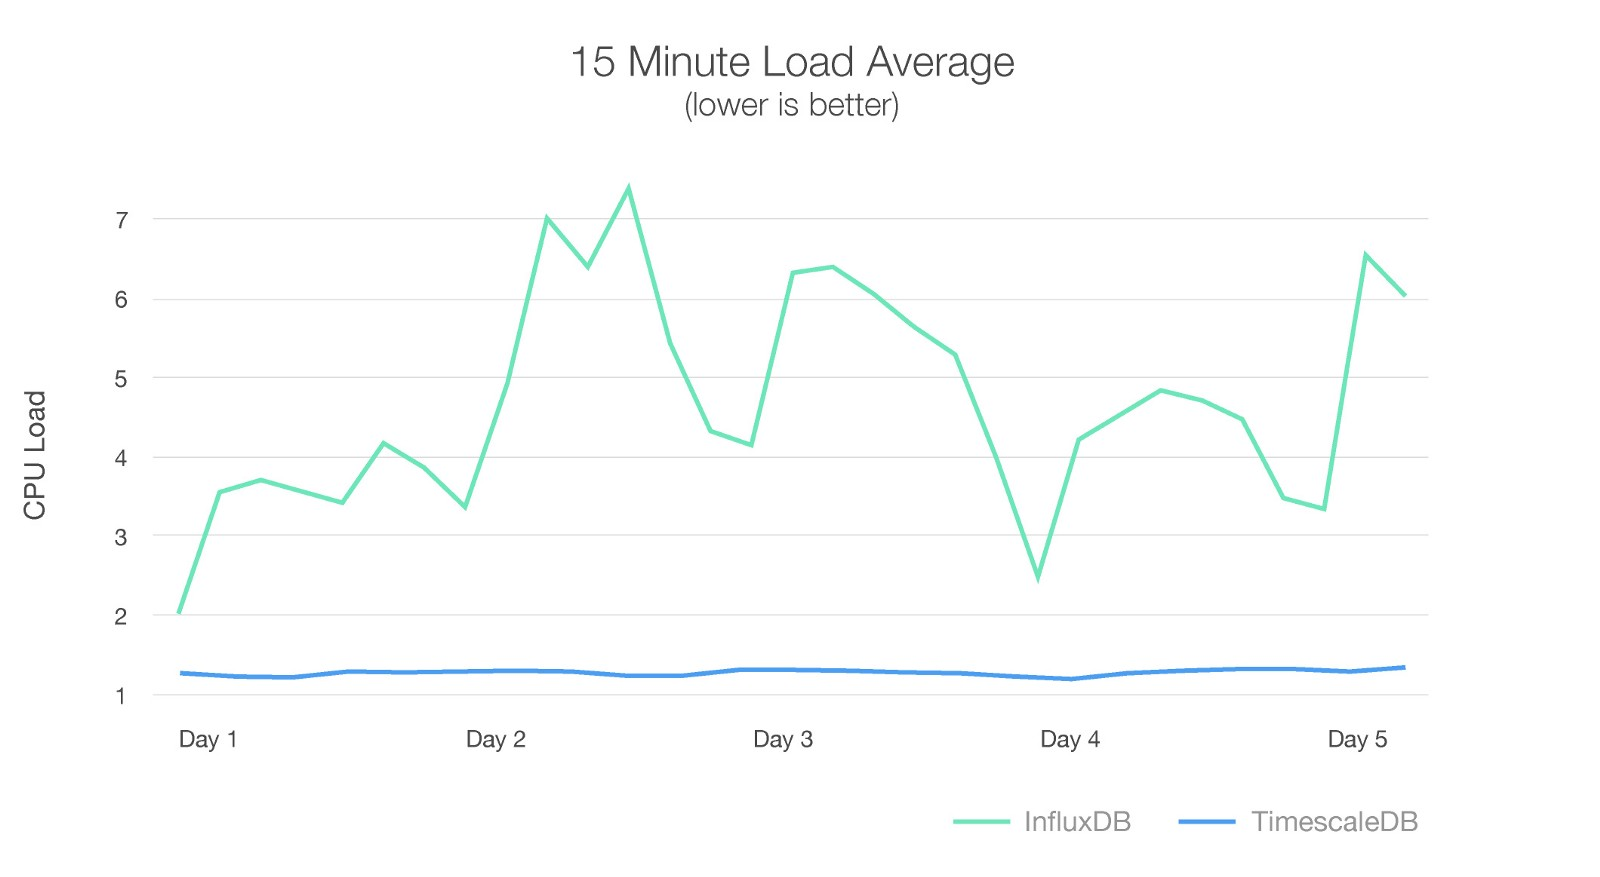
\includegraphics[width=\textwidth]{latex/figures/cpu_load_influx_ts.png}
                \caption[CPU utilization]{CPU utilization}
                \label{fig:cpu_db}
            \end{subfigure}
            \begin{subfigure}[b]{0.49\textwidth}
                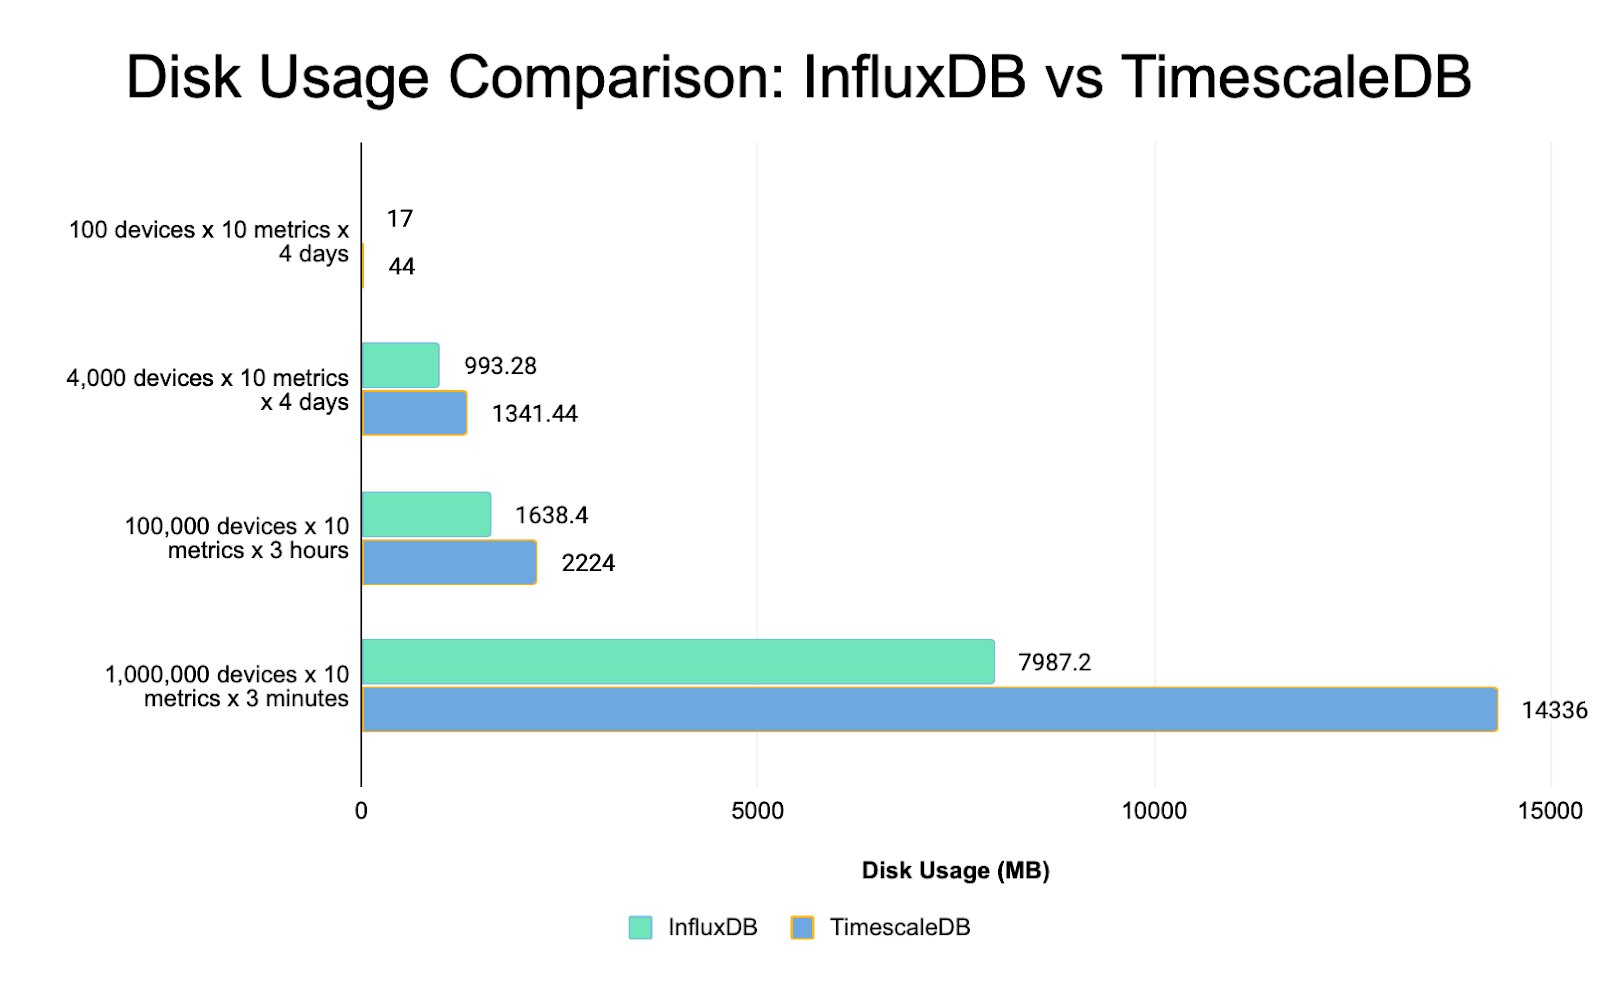
\includegraphics[width=\textwidth]{latex/figures/diskusage_influx_ts.png}
                \caption[Disk Usage]{Disk Usage}
                \label{fig:disk_db}
            \end{subfigure}
            \caption[Resource consumption of InfluxDB and TimescaleDB]{Resource consumption of InfluxDB and TimescaleDB modified after \cite{freedman_timescaledb_2020}}
        \end{figure}
        
        \begin{figure}[h!]
            \centering
            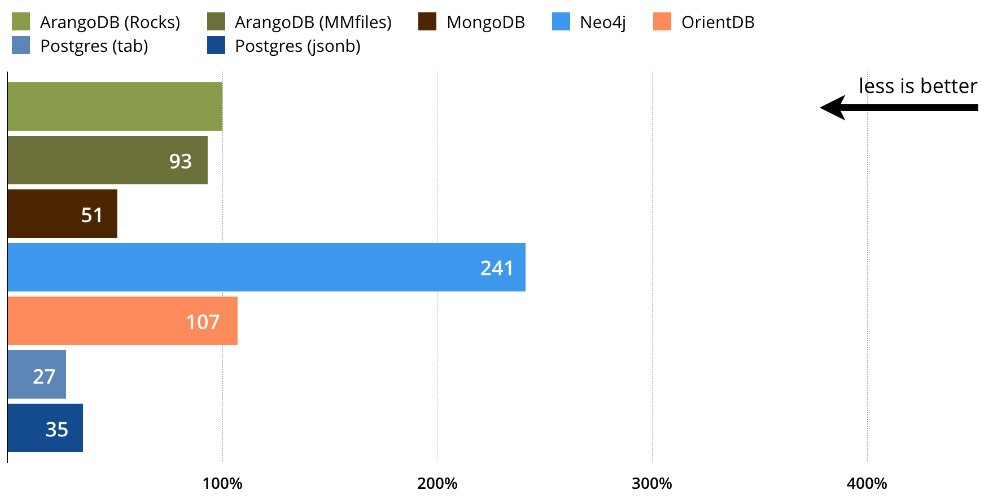
\includegraphics[width=\textwidth]{latex/figures/mem_db.jpg}
            \caption[Memory consumption of relational databases]{Memory consumption of relational databases \cite{noauthor_benchmark_2018}}
            \label{fig:mem_db}
        \end{figure}
        
        
        The number one web application security risk is command injection.
        An injection occurs, when user data is processed by an application and interpreted as part of the command. This may lead to unauthorized data access or damage of the stored data. 
        The user input could contain an escape sequence and an SQL command to access data stored in an SQL-database.\\
        
        \newpage
        
        To protect an application against SQL injections, the Open Web Application Security Project (OWASP) provides four possible defenses in \cite{owasp_foundation_sql_2021}.
        \begin{itemize}
            \item Prepared Statements
            \item Stored procedures
            \item Input validation with allow-lists 
            \item Input escaping for all user supplied data
        \end{itemize}
        
        Prepared statements are also known as parameterized queries and use a query with predefined SQL code, which is compiled on the first execution and reused on every later execution. Each parameter is passed to the SQL separately and wont be run as SQL code, even if escape sequences are encountered.  This is the safest way to handle user provided input and should be used if possible \cite{owasp_foundation_sql_2021}, \cite{benita_preventing_2021}. As input escaping is the most fragile solution, it should only be used in addition to the other solutions, or as last resort, if none of the other solutions are applicable \cite{owasp_foundation_sql_2021}. 
        
%
\newpage

%%%%%%%%%%%%%%%%%%%%%%%%%%%%%%%%%%%%%
%%%%%%%%%%%%%%%%%%%%%%%%%%%%%%%%%%%%%
%%%%%%%%%%%%   SECTION   %%%%%%%%%%%%
%%%%%%%%%%%%%%%%%%%%%%%%%%%%%%%%%%%%%
%%%%%%%%%%%%%%%%%%%%%%%%%%%%%%%%%%%%%
\section{Evaluation Setup}
\label{sec:measurement:eval_setup}
%
    As we gave some general recommendations, we are talking about our collection setup next.
    We provide a short guide on the server hardening steps taken on the collection server. A presentation of our implementation follows this.
    
    \subsection{Server}
        \label{subsec:measure:server}
        We use an Ubuntu 20.4 operating system with Security Enhanced Linux (SELinux) \cite{noauthor_what_nodate-1} enabled for the server.
        Ubuntu is a well known stable distribution, which provides the security and stability needed for a server. SELinux uses policies to define access controls for applications, processes and files \cite{noauthor_what_nodate-1}. This increases the barrier for a possible intruder to exploit our system.\\
        
        To harden the server against user enumeration and login brute-forcing, we assign an individual username and disable root login. Next, we allow login only with ssh keys, which are secured with passwords.
        Further we strengthen the server with \textit{fail2ban} and configure it to ban IPs based on failed login attempts and user name retries over time. It uses \textit{iptables} rules to block IPs. Furthermore, we configure the firewall to drop all packages except for SSH and port 53 (DNS).\\
        
        The server application is run in a Linux container for additional separation. We reduced the number of packages to only those needed to run our application and the security measurements, reducing the number of exploitable applications on the system. The containerization adds another layer of security, as an adversary would need to escape the container first, before he can compromise the host system. In case of a successful attack, only the container needs to be disposed and the data sanitized, instead of the whole server.
        
    \subsection{Implementation}
        \label{subsec:measure:implementation}
        As we provide a reference implementation for the collection tool, we also provide a basic implementation for the collection server \cite{venz_ikstreamdns-handler_2021}. It is written in Python, as it is easy to read and reproduce in different languages. Furthermore, it can be used for fast prototyping with a wide range of libraries.\\
        We implemented the server as a multithreaded data handler. The thread-safe queue library is used to pass data between the different threads. The main thread listens to incoming UDP data on port 53. First a check is executed if the received data is a valid DNS query. If the domain and subdomain match our collection subject, the data is put in a queue for the processing thread, otherwise the data is dropped.\\
        This helps to reduce processing overhead, and filling up the queue with data, that doesn't matter to the collection.
        The processing pulls data from the data-queue as soon as it is accessible. The ID, message number, and total message count are extracted from the query string. 
        If the ID matches with already present messages, it is checked if the message is older than two minutes and the old data discarded in that case. We decided to allow some time to pass before the whole message is expected. This makes up for network congestion or a resolver under high load.\\
        If a message number already exists for the ID, the older message is kept and the new one discarded. This may occur if the DNS response didn't reach the client in time and the same query has been send again. The data-queue element is marked as done after the processing to free up space in the data-queue. If all messages of an ID arrived, the user-data object is put into the user-processing-queue and removed from the list of user-data processed by the thread.
        An user-data object consists of the ID, a dictionary of message with their message number and the time stamp of the last received message.\\
        The user thread checks the user queue for new data constantly. When a new user-data object is detected on the queue, all stored messages are combined into one string.
        As the original messages has been encoded base 16 before transmission, the first step is to decode the string. The resulting base 64 encoded string is also decoded and stored as raw bytes in a file. These raw bytes are decrypted with \textit{Openssl} using the matching private key. 
        The server version 0.1.1 stores the user data in files, named after the user id with a timestamp as first column. Version 0.2.1 is intended to use a database as storage backend and allow additional ID encryption. This was chosen for the ease of prototyping and testing the performance of the data processing.
        As data is stored locally only, code injections, like SQL injections are no concern for the current version. 

%
%%%%%%%%%%%%%%%%%%%%%%%%%%%%%%%%%%%%%
%%%%%%%%%%%%%%%%%%%%%%%%%%%%%%%%%%%%%
%%%%%%%%%%%%   SECTION   %%%%%%%%%%%%
%%%%%%%%%%%%%%%%%%%%%%%%%%%%%%%%%%%%%
%%%%%%%%%%%%%%%%%%%%%%%%%%%%%%%%%%%%%
\section{Summary}
We discussed some general recommendations for server security and data storage in the last chapter. We also provided an overview of our collection setup and dalec-server implementation. In the next chapter we will provide some information on tests we performed to check what our implementation is possible to do. We will also discuss the limitations of our setup in the following chapter.

%
